\documentclass[pdflatex,sn-mathphys-num]{sn-jnl}

\usepackage{graphicx}
\usepackage{amsmath,amssymb,amsthm}
\usepackage[ruled]{algorithm2e}
\usepackage{array,booktabs,longtable}
\usepackage{microtype}
\usepackage{url}
\usepackage{xcolor}
% sn-jnl loads hyperref; configure it without reloading the package.
% hypertexnames=false prevents duplicate anchors inherited from frozen
% section files that restart local equation numbering.
\hypersetup{hidelinks,hypertexnames=false,pdfauthor={Jeng-Shyang Pan; Peng-Yu Duan; Li-Fa Liu; Qing-Yong Yang; Shu-Chuan Chu}}
\graphicspath{{figures/}}
\setlength{\emergencystretch}{3em}
\raggedbottom

\newcommand{\Description}[1]{}
% Compatibility alias for the IEEEtran appendix entry point in the frozen section.
\renewcommand{\appendices}{\appendix}
\newtheorem{proposition}{Proposition}

\begin{document}

\title[Outcome-Aligned Task Offloading]{Outcome-Aligned Task Offloading for DNN Inference in Heterogeneous Fog Networks}

\author[1,2]{\fnm{Jeng-Shyang} \sur{Pan}}\email{100112@nuist.edu.cn}
\author[1]{\fnm{Peng-Yu} \sur{Duan}}\email{202483060107@sdust.edu.cn}
\author[1]{\fnm{Li-Fa} \sur{Liu}}\email{202282060085@sdust.edu.cn}
\author[1]{\fnm{Qing-Yong} \sur{Yang}}\email{yang\_qy@sdust.edu.cn}
\author*[3]{\fnm{Shu-Chuan} \sur{Chu}}\email{100130@nuist.edu.cn}

\affil[1]{\orgname{College of Computer Science and Engineering, Shandong University of Science and Technology},
  \orgaddress{\city{Qingdao}, \postcode{266590}, \country{China}}}
\affil[2]{\orgname{Department of Information Management, Chaoyang University of Technology},
  \orgaddress{\city{Taichung}, \postcode{41349}, \country{Taiwan}}}
\affil[3]{\orgname{School of Artificial Intelligence, Nanjing University of Information Science and Technology},
  \orgaddress{\city{Nanjing}, \postcode{210044}, \country{China}}}

\abstract{Heterogeneous fog clusters must place DNN inference requests under coupled compute, memory, communication, and deadline constraints. We study a practical mismatch between candidate search and deployed service: evolutionary schedules are often ranked before feasibility repair, although only the repaired schedule is executed. M-CA-ALM resolves this mismatch by ranking repaired phenotypes while retaining unrepaired genotypes for variation and by applying guarded augmented-Lagrangian refinement. In a frozen five-node benchmark with 30 paired seeds, satisfaction improves over GA-Hybrid by 0.72--5.28 percentage points at congested scales $N=120$--$300$. An independent GA-family test reproduces a 3.08-point repair-aware gain, while a split-isolated OfflineGNN remains 9.67 points lower after equal scale averaging. In separate 500-slot replay experiments at $N=180$, mean satisfaction increases from 33.45\% to 46.41\% and median queue saturation is delayed from slot 7 to slot 56. The advantage disappears at the immediate-overload boundary where all controllers saturate by slot 2. These results support outcome-aligned selection within the tested five-node simulator and do not establish cross-topology or deployment generalization.}
\keywords{Fog computing, mobile edge computing, DNN inference, task offloading, repair-aware optimization, congestion-aware scheduling}

\maketitle

\section{Introduction}

Latency-sensitive DNN inference increasingly relies on small fog clusters whose nodes differ in compute speed, memory, and communication quality. The scheduler must choose one node per request while respecting deadlines and resource limits. This discrete problem becomes difficult near congestion, where moving one task can change queueing and context-switching costs for many others \cite{Mao2017}.

Practical schedulers commonly separate candidate generation from feasibility enforcement. An optimizer first proposes a complete assignment, after which a repair operator reassigns or rejects tasks that violate memory, load, or deadline checks. This architecture is operationally useful, but it creates an objective mismatch: search is often ranked on raw assignments even though only repaired assignments are deployed. Our audit of the original pipeline showed that this mismatch can dominate the comparison. Raw GA-Hybrid and M-CA-ALM assignments agreed on only 23.1\% of task-node choices, whereas agreement rose to 60.8\% after shared repair. Consequently, a method may appear different internally while producing nearly identical service outcomes.

This paper addresses that mismatch directly. We propose an outcome-aligned version of the Memetic Congestion-Aware Augmented Lagrangian Method (M-CA-ALM). Candidate genotypes remain unrepaired to preserve population diversity, but elite selection evaluates the phenotype obtained after the same deterministic feasibility operator used at deployment. Augmented-Lagrangian local refinement is guarded: a refined candidate replaces its parent only when it improves a feasibility-first lexicographic criterion. The resulting search therefore optimizes the measured service outcome without collapsing the whole population into repaired copies.

The paper makes three contributions:
\begin{itemize}
    \item \textbf{Outcome-aligned memetic selection.} We introduce repair-aware phenotype ranking with non-Lamarckian genotype preservation, aligning candidate selection with final satisfied-task count while retaining structurally distinct candidates.
    \item \textbf{Guarded congestion-aware refinement.} We combine integer evolutionary exploration with sigmoid-relaxed ALM updates and accept a local update only when it improves feasibility first and satisfaction second.
    \item \textbf{A reproducible static-to-replay evaluation.} We fix the metric implementation and solver configuration, combine 30 paired static seeds with state-preserving replay, test repair-aware transfer in an independent GA family, and include a split-isolated offline graph policy. Paired tests, Holm correction, confidence intervals, and paired effect sizes are reported throughout.
\end{itemize}

The evidence supports a deliberately bounded claim. We call a load ``recoverable congestion'' when state-preserving replay retains a nonzero interval before the backlog reaches its cap. The ``immediate-overload boundary'' is the regime in which all tested controllers reach the cap at the same early slot. M-CA-ALM does not improve an already solved light-load regime. Its benefit appears in recoverable congestion, where it improves repaired satisfaction without sacrificing resource feasibility, at the cost of higher runtime. Formal replay confirms stronger service persistence at $N=180$. At the immediate-overload boundary at $N=300$, M-CA-ALM shows no reproducible advantage. Static experiments, independent transfer tests, and state-preserving replay are separate evidence tiers and are not pooled into one summary estimate. All conclusions are therefore limited to the fixed five-node simulator and tested load regimes; no cross-infrastructure, online-stability, capacity-planning, or hardware-deployment claim is made.

\section{Related Work}

\subsection{Mobile Edge Computing and Fog Computing Architectures}
Mobile Edge Computing (MEC) and Fog Computing extend cloud resources toward geographically distributed edge nodes so that latency-sensitive services can be executed closer to end users \cite{Mao2017, Shi2016}. Surveys by Mach et al. \cite{Mach2017} and Abbas et al. \cite{Abbas2018} establish the architectural motivation: lower round-trip latency, better bandwidth locality, and improved support for IoT-scale service density. In fog settings, task-offloading surveys summarize how workloads are distributed across heterogeneous edge resources \cite{Kumari2022}, while edge-intelligence studies further connect resource orchestration with AI inference and decision support \cite{Zhou2019}.

These architectural studies motivate the present work but do not by themselves resolve the control problem addressed here. Once a heterogeneous fog tier is fixed, the main challenge shifts to how a controller allocates model-specific tasks under hard memory limits, unequal compute capacities, fluctuating communication costs, and repeated congestion.

\subsection{Computation Offloading Optimization}
Task offloading has long been formulated as a latency-minimization, energy-minimization, or utility-maximization problem. Early binary-decision models typically decide whether a task should remain local or be offloaded, often under simplified service assumptions \cite{Zhang2016}. Later work broadened the formulation toward multi-user and heterogeneous settings, including energy-aware allocation and joint communication--computation optimization \cite{Chen2018, You2017, Liu2016, Bi2018, Zhou2019, Deng2020}. Representative studies also consider IoT-oriented edge placement, security-aware offloading, and user-centric offloading \cite{Sun2016, Premsankar2018, Samy2022, Deng2021}. These works motivate constrained offloading, but they do not evaluate the repair-aware evolutionary selection question considered here.

However, much of this literature still targets one-shot or slot-local objectives and often evaluates schedulers primarily by energy or average delay. That perspective is useful but incomplete for repeated DNN service, where the scheduling decision in one slot can shape backlog, tail latency, and admission quality in later slots.

\subsection{Deep Learning Inference at the Edge}
Edge-side DNN inference introduces system properties that make offloading harder than generic task scheduling. Neurosurgeon, Edgent, and BottleNet respectively demonstrate partitioning, on-demand co-inference with early exiting, and intermediate-feature compression across device, edge, and cloud resources \cite{Kang2017, Li2018, Eshratifar2019}. Distributed inference and adaptive DNN surgery further show that the execution graph and hardware setting can affect the offloading decision \cite{Teerapittayanon2017, Hu2019DNNsurgery}.

For the scheduling problem studied here, the key implication is that DNN jobs are not interchangeable scalar loads. Different models generate different latency traces and memory footprints, which makes congestion-sensitive placement substantially more difficult than allocating homogeneous service requests.

\subsection{AI-Driven Optimization (DRL)}
Deep Reinforcement Learning (DRL) is a natural candidate for dynamic offloading because it can, in principle, optimize a long-horizon objective directly. DQN-style methods \cite{Mnih2015} and later DRL formulations have been adapted to MEC scheduling and task offloading \cite{Huang2020, Tang2022}. Their main appeal is that they can absorb non-stationarity and multi-step reward structure without requiring an exact analytical model.

The difficulty is operational rather than conceptual. DRL policies often require large training effort, careful reward shaping, and explicit safety handling once hard feasibility constraints are introduced. When infrastructure conditions change quickly, the distinction between ``policy quality'' and ``policy retraining burden'' becomes important. This is why snapshot-rerunnable optimization baselines remain relevant even when the evaluation target includes long-horizon behavior.

\subsection{Gap Analysis}
Table \ref{tab:related_work} summarizes the comparison between the present study and representative prior categories. The distinguishing point is not that this paper is the first to study offloading, congestion, or learning. Rather, it combines several ingredients that are usually evaluated separately:
\begin{itemize}
    \item \textbf{Batch-consistent congestion modeling:} Instead of importing a steady-state queue as the main optimization target, the simulator uses a static batch congestion penalty with explicit context-switching overhead so that the search signal remains aligned with snapshot scheduling.
    \item \textbf{State-preserving long-horizon evaluation:} The replay carries unresolved task identities across slots and applies admission-aware scoring under repeated control. The 500-slot experiment quantifies both recoverable congestion and the immediate-saturation boundary instead of extrapolating static rankings to dynamic service.
    \item \textbf{Shared feasibility enforcement across all methods:} Final schedules are passed through the same Safe Harbor Repair rule, which makes the comparison about optimization quality in a common admissible decision space rather than about who tolerates more hidden infeasibility.
    \item \textbf{An auditable evidence ladder:} The completed evidence links metric audits, repair-collapse diagnosis, fixed-capacity congestion sweeps, state-preserving replay, and paired statistical tests under one frozen implementation. Deployment validation remains a separate extension.
\end{itemize}

\begin{table*}[t]
\caption{Positioning of the present study against representative prior work categories}
\label{tab:related_work}
\centering
\small
\setlength{\tabcolsep}{3pt}
\begin{tabular}{p{0.15\textwidth}p{0.25\textwidth}p{0.25\textwidth}p{0.25\textwidth}}
\toprule
\textbf{Work} & \textbf{Decision and objective} & \textbf{Feasibility treatment} & \textbf{Reported evidence} \\
\midrule
Zhang et al. \cite{Zhang2016} & Binary offloading; energy efficiency & Penalty-based constraints & Snapshot simulation \\
Meng et al. \cite{Meng2019} & Partial offloading; delay minimization & Closed-form analytical policy & Analytical evaluation \\
Min et al. \cite{Min2019} & Binary offloading; energy-aware control & Policy-dependent handling & Learned dynamic policy and simulation \\
\textbf{Ours} & \textbf{Binary fog assignment; repaired service satisfaction} & \textbf{Shared final repair for every compared method} & \textbf{Frozen benchmark with 30 paired static seeds and 20 paired 500-slot replay runs} \\
\bottomrule
\end{tabular}
\end{table*}

\section{System Model and Problem Formulation}

\subsection{Fog Computing Network Architecture}
The implemented simulator considers a centralized scheduler and a heterogeneous set of fog nodes $\mathcal{F}=\{1,\dots,F\}$. The standard benchmark is a one-shot batch placement problem, while the dynamic extension repeats the same placement pipeline over a sequence of decision slots. In both cases, the current codebase models fog execution only: each task is either assigned to one fog node or later rejected by the feasibility repair stage if no safe placement exists. The resulting formulation is therefore a constrained fog-selection problem rather than a joint local--edge--cloud formulation.

\subsection{Task Model and Binary Offloading}
Each request corresponds to one DNN inference task. In slot $t$, the scheduler observes an active task set $\Omega_t$ that contains newly arrived requests together with any unresolved backlog carried from the previous slot. Each task $i \in \Omega_t$ is represented by a task type and a deadline,
\begin{equation}
    \mathcal{T}_i = \{\tau_i, T_i^{\max}\},
\end{equation}
where $\tau_i \in \{1,2,3\}$ denotes VGG16, ResNet50, or MobileNetV2, respectively. The detailed communication and computation costs are not generated from a symbolic workload formula inside the optimizer; instead, they are obtained from precomputed matrices derived from hardware profiles. Let
\begin{equation}
    x_{i,f}(t) \in \{0,1\}
\end{equation}
denote the assignment decision, with $x_{i,f}(t)=1$ when task $i$ is mapped to fog node $f$ in slot $t$. We also define an explicit admission indicator
\begin{equation}
    a_i(t) \in \{0,1\},
\end{equation}
where $a_i(t)=1$ means that task $i$ remains assigned after repair and $a_i(t)=0$ means that the final repaired schedule rejects the task. Before repair, the optimizer produces exactly one node choice per active task:
\begin{equation}
    \sum_{f \in \mathcal{F}} x_{i,f}(t)=1,\quad \forall i \in \Omega_t.
\end{equation}
After repair, some tasks may be dropped, which is represented in the evaluation code by an all-zero row and therefore satisfies
\begin{equation}
    \sum_{f \in \mathcal{F}} x_{i,f}(t)=a_i(t),\quad \forall i \in \Omega_t.
\end{equation}

\subsection{Profile-Driven Cost Model}
For each active task-node pair $(i,f)$, the simulator precomputes:
\begin{itemize}
    \item $\mathrm{Comp}_{i,f}$: base execution time obtained from the model profile and node capability;
    \item $\mathrm{Comm}_{i,f}$: uplink transmission time computed from the wireless link model.
\end{itemize}
This design matches the implementation in which the optimization routines operate on the matrices stored in the structure $\mathrm{Pre}$.

\subsection{Communication and Transmission Model}
The communication between end users and fog nodes follows an OFDMA-style uplink model. The achievable data rate from user $i$ to fog node $f$ is
\begin{equation}
    R_{i,f} = B_{i,f} \log_2 \left( 1 + \frac{P_i^{tx} |h_{i,f}|^2}{\sigma^2 + I_{i,f}} \right)
\end{equation}
and the communication delay is
\begin{equation}
    T_{i,f}^{comm} = \frac{D_i}{R_{i,f}}.
\end{equation}
In practice, these values are already encoded in $\mathrm{Comm}_{i,f}$ by the preprocessing routine.

\subsection{Computation Model with Static Batch Congestion Penalty}
The simulator penalizes overloaded nodes by combining a static batch congestion term with an explicit context-switching overhead. Let
\begin{equation}
    L_f(t) = \sum_{i \in \Omega_t} x_{i,f}(t)\,\mathrm{Comp}_{i,f}
\end{equation}
be the aggregate compute load on node $f$ in slot $t$, and let $\bar{T}_t=\frac{1}{|\Omega_t|}\sum_{i \in \Omega_t} T_i^{\max}$ be the mean task deadline used as a normalization window. The effective utilization is
\begin{equation}
    \rho_f(t) = \frac{L_f(t)}{\bar{T}_t}.
\end{equation}
The congestion multiplier used in the code is
\begin{equation}
    q_f(t) =
    \begin{cases}
        1 + \dfrac{\rho_f(t)}{2(1-\rho_f(t)+\epsilon)}, & \rho_f(t) < 0.99,\\
        10^4, & \rho_f(t) \ge 0.99,
    \end{cases}
\end{equation}
where $\epsilon$ is a small numerical stabilizer. Let $K_f(t)=\sum_{i \in \Omega_t} x_{i,f}(t)$ denote the number of tasks assigned to node $f$. The context-switching overhead applied to all tasks on node $f$ is
\begin{equation}
    T_f^{ctx}(t) = \alpha_{ctx} K_f(t)^2,
\end{equation}
with $\alpha_{ctx}=500\mu s$. Therefore, the end-to-end latency of task $i$ placed on node $f$ is
\begin{equation}
    T_i(f,t) = \mathrm{Comm}_{i,f} + \mathrm{Comp}_{i,f}\, q_f(t) + T_f^{ctx}(t).
\end{equation}
This is the latency model actually used by the evaluation code.

\subsection{Resource Feasibility}
Each fog node has a memory budget $M_f^{cap}$. The memory footprint of task $i$, denoted by $m_i$, is approximated from the corresponding DNN profile. A placement is treated as resource-feasible by the simulator when
\begin{equation}
    \sum_{i \in \Omega_t} x_{i,f}(t) m_i \le M_f^{cap}, \quad \forall f \in \mathcal{F},
\end{equation}
and the congestion indicator remains below the safety threshold used by the simulator. If a candidate placement violates these limits, the repair stage reassigns or drops tasks until the returned solution becomes resource-feasible.

\subsection{Dynamic Rollout Semantics}
\label{sec:dynamic_rollout}
Rather than treating each batch as an isolated placement instance, we interpret the simulator as a repeated closed-loop controller operating over a horizon of $H$ decision slots. The implemented solver in each slot is still the repaired static optimizer, but its input state, feasible region, and realized utility are coupled through backlog carry-over and environment perturbations. Let $A_t$ denote the number of new arrivals in slot $t$, and let $Q_t$ denote the backlog carried into that slot. The active set size is therefore
\begin{equation}
    |\Omega_t| = A_t + Q_t.
\end{equation}
We summarize the controlled system state by
\begin{equation}
    S_t = \left(Q_t,\Omega_t,\mathcal{C}_t,\xi_t\right),
\end{equation}
where $\mathcal{C}_t$ collects the communication and computation cost matrices used by the current slot, and $\xi_t$ represents exogenous perturbations such as bursty arrivals, deadline tightening, communication inflation, or node-capacity degradation. For a given state, the controller chooses a repaired binary assignment $\mathbf{X}(t)=\{x_{i,f}(t)\}$. After evaluation, unresolved tasks are transferred to the next slot through
\begin{equation}
    Q_{t+1} = \min\left\{Q^{\max}, \sum_{i \in \Omega_t} \left(1-US_i(t)\right)\right\},
\end{equation}
where $Q^{\max}$ is the backlog cap used by the rollout script. The resulting closed-loop transition can be written compactly as
\begin{equation}
    S_{t+1} = \Phi\!\left(S_t,\mathbf{X}(t),\xi_{t+1}\right).
\end{equation}
The state-preserving replay implementation invokes the same slot-level optimizer repeatedly and retains unresolved task identities between slots. The formal replay reported in Section~5 uses 20 paired environment runs at each stress scale and validates complete algorithm pairing, environment seeds, slot coverage, and queue-state continuity before analysis.

\subsection{User Satisfaction (US), Dynamic Metrics, and Problem Formulation}
\label{sec:problem}
For optimization, we use a smooth surrogate of deadline satisfaction:
\begin{equation}
    \widetilde{US}_i(T_i(t)) = \frac{1}{1 + \exp(\nu (T_i(t) - T_i^{\max}))}.
\end{equation}
For reporting, however, the simulator uses a strict binary score:
\begin{equation}
    US_i(t)=
    \begin{cases}
        1, & \text{if } T_i(t) \le T_i^{\max} \text{ and resource-feasible},\\[2pt]
        0, & \text{otherwise}.
    \end{cases}
\end{equation}
For a single slot, the practical objective of the discrete solver before repair is
\begin{subequations}
\begin{align}
    \max_{\mathbf{X}(t)} \quad & \sum_{i \in \Omega_t} US_i(t) \\
    \text{s.t.} \quad & \sum_{f \in \mathcal{F}} x_{i,f}(t) = 1, \quad \forall i \in \Omega_t, \\
    & \sum_{i \in \Omega_t} x_{i,f}(t) m_i \le M_f^{cap}, \quad \forall f, \\
    & \rho_f(t) < 0.99, \quad \forall f, \\
    & x_{i,f}(t) \in \{0,1\}.
\end{align}
\end{subequations}
The repair stage is part of the implemented decision pipeline, so the evaluated solution is the repaired binary assignment rather than the raw optimizer output. For the dynamic rollout, we do not claim that the current solver directly optimizes a long-horizon objective. Instead, we evaluate repeated closed-loop behavior through rollout-level metrics:
\begin{equation}
    \max_{\{\mathbf{X}(t)\}_{t=1}^{H}} \quad \mathcal{J}_H = \sum_{t=1}^{H} \gamma^{t-1}\!\left[\sum_{i \in \Omega_t} U_i(t) - \lambda_Q Q_{t+1}\right],
\end{equation}
where $\gamma \in (0,1]$ is a horizon-weighting factor and $\lambda_Q \ge 0$ penalizes backlog accumulation. This long-horizon objective is used as an organizing principle: even though the implemented controller solves slot-local subproblems, the repeated rollout is evaluated by how well it maintains timely service while suppressing future backlog. To make this interpretation measurable, we export the following trajectory summaries:
\begin{align}
    \overline{US} &= \frac{1}{H}\sum_{t=1}^{H}\frac{1}{|\Omega_t|}\sum_{i \in \Omega_t} US_i(t),\\
    \overline{Q} &= \frac{1}{H}\sum_{t=1}^{H} Q_{t+1},\\
    Q^{\mathrm{AUC}} &= \sum_{t=1}^{H} Q_{t+1},\\
    Q^{\max} &= \max_{1 \le t \le H} Q_{t+1},\\
    \overline{A} &= \frac{1}{H}\sum_{t=1}^{H}\frac{1}{|\Omega_t|}\sum_{i \in \Omega_t} a_i(t),
\end{align}
where $H$ is the rollout length. In addition, the evaluation script reports the final backlog $Q_{H+1}$, together with rollout-level latency percentiles such as P95 and P99 over all admitted tasks. These metrics let the unified long-horizon controller viewpoint separate three effects that are conflated in a static snapshot: immediate deadline satisfaction, carried congestion passed to future slots, and the conservativeness of the repaired admission decisions.

For the admission-aware and failure-aware variants, the code evaluates a slot-level utility that explicitly distinguishes timely admission, late admission, and outright rejection. Let
\begin{equation}
    z_i(t) = a_i(t)\,US_i(t)
\end{equation}
denote the indicator that task $i$ is both admitted and completed within deadline, and define the normalized excess-delay ratio
\begin{equation}
    \delta_i(t) = \max\left\{\frac{T_i(t)}{T_i^{\max}} - 1, 0\right\}.
\end{equation}
The admission-aware utility used by the new dynamic post-processing stage is
\begin{equation}
\begin{aligned}
    U_i(t) ={}& \omega_{\mathrm{on}} z_i(t) - \omega_{\mathrm{late}} a_i(t)\left(1-z_i(t)\right) \\
    &- \omega_{\mathrm{ex}} a_i(t)\delta_i(t) - \omega_{\mathrm{drop}}\left(1-a_i(t)\right),
\end{aligned}
\end{equation}
where the current configuration uses $(\omega_{\mathrm{on}}, \omega_{\mathrm{late}}, \omega_{\mathrm{ex}}, \omega_{\mathrm{drop}}) = (1.0, 0.60, 0.24, 0.22)$. The rollout export then reports
\begin{align}
    \overline{A}_{\mathrm{timely}} &= \frac{1}{H}\sum_{t=1}^{H}\frac{1}{|\Omega_t|}\sum_{i \in \Omega_t} z_i(t),\\
    \overline{A}_{\mathrm{late}} &= \frac{1}{H}\sum_{t=1}^{H}\frac{1}{|\Omega_t|}\sum_{i \in \Omega_t} a_i(t)\left(1-z_i(t)\right),\\
    \overline{D} &= \frac{1}{H}\sum_{t=1}^{H}\frac{1}{|\Omega_t|}\sum_{i \in \Omega_t} \left(1-a_i(t)\right),\\
    \overline{U} &= \frac{100}{H}\sum_{t=1}^{H}\frac{1}{|\Omega_t|}\sum_{i \in \Omega_t} U_i(t).
\end{align}
These additional metrics are not meant to replace $\overline{US}$ or backlog summaries. Instead, they provide a more discriminative diagnostic for unified long-horizon control: two policies may admit a similar number of tasks in the current slot, yet differ sharply in whether that admission remains timely, whether it amplifies future backlog, and whether it degrades gracefully under dynamic node failures.

\section{Outcome-Aligned M-CA-ALM}

\subsection{Motivation}
Let $\mathbf{X}$ denote an integer task-to-node assignment and let $\mathcal{R}(\mathbf{X})$ denote the deterministic Safe Harbor repair operator. The reported objective is evaluated on $\mathcal{R}(\mathbf{X})$, not on $\mathbf{X}$. Ranking candidates only by a raw surrogate can therefore select a genotype whose deployed phenotype serves fewer tasks. M-CA-ALM closes this gap by using repaired outcomes for selection while retaining raw genotypes for variation.

\subsection{Population and Local Relaxation}
Each individual stores one node index per task and is generated in a fixed order: one greedy genotype is inserted first, perturbed copies are created by changing a small number of task--node genes, and the remaining individuals are sampled uniformly over admissible nodes. This genotype is the object passed to crossover and mutation. For local refinement, an integer gene is mapped to logits $\mathbf{Z}$ and probabilities
\begin{equation}
 p_{i,f}=\frac{\exp(z_{i,f})}{\sum_{j\in\mathcal{F}}\exp(z_{i,j})}.
\end{equation}
The hard deadline indicator is approximated during refinement by
\begin{equation}
 \widetilde{US}_i=\left[1+\exp\left(\nu(T_i-T_i^{\max})\right)\right]^{-1}.
\end{equation}
The ALM gradient includes the load-dependent multiplier $q_f(\rho_f)$ from Section~3, so the marginal cost increases as a node approaches the stability boundary.

\subsection{Repair-Aware Non-Lamarckian Selection}
For candidate $\mathbf{X}$, selection constructs a temporary phenotype
\begin{equation}
 \widehat{\mathbf{X}}=\mathcal{R}(\mathbf{X})
\end{equation}
and computes its binary satisfied-task count. The repaired phenotype is used only for scoring. It is not written back to the genotype. This distinction is essential: phenotype ranking aligns selection with deployment, while genotype preservation prevents deterministic repair from making the population structurally homogeneous.

Candidates are compared lexicographically. A resource-feasible phenotype dominates an infeasible phenotype; between feasible phenotypes, the larger satisfied-task count wins; between infeasible phenotypes, lower violation wins before satisfaction is considered. The same rule guards ALM local refinement, so a locally refined child cannot replace a strictly better parent. The repaired phenotype is temporary: it is used for phenotype ranking and for the ALM child-acceptance test, but it never overwrites the genotype. Only after the final elite has been selected is the shared repair and discrete post-optimization executed to produce the deployed schedule.

\begin{algorithm}[t]
\caption{Outcome-Aligned M-CA-ALM}
\label{alg:mca_official}
\SetAlgoLined
\KwIn{Task set, fog nodes, population size $P$, generations $G$}
\KwOut{Feasible repaired assignment}
Initialize greedy, perturbed, and random integer genotypes\;
\For{$g=1$ \KwTo $G$}{
  \ForEach{genotype $\mathbf{X}$}{
    Optionally generate $\mathbf{X}'$ by short ALM refinement\;
    Temporarily repair $\mathbf{X}$ and $\mathbf{X}'$ for scoring\;
    Accept $\mathbf{X}'$ only if its repaired lexicographic score improves\;
    Rank $\mathbf{X}$ using the temporary phenotype $\mathcal{R}(\mathbf{X})$\;
    Keep the unrepaired genotype for variation\;
  }
  Apply tournament selection, crossover, mutation, and elitism\;
}
Apply shared repair and discrete post-optimization only to the selected elite\;
\Return the final assignment\;
\end{algorithm}

\subsection{Implementation contract}
The shared Safe Harbor Repair (SFR) is deterministic. It sorts tasks by ascending minimum computation time and tests each task on its original node. The original node is retained only when memory fits, the post-placement load satisfies $\rho_f<0.95$, and latency including the context term $500\times10^{-6}n_f^2$ meets the deadline. If that test fails, all nodes are scanned in ascending index order and the feasible node with the lowest estimated latency is selected. If no node is feasible, the task is dropped. The load multiplier uses a $10^{-6}$ stabilizer; the reported metric still treats $\rho_f\geq0.99$ as a resource violation. Thus the repair threshold and evaluation threshold are distinct.

The formal call path passes ``use\_repair=false'' to the internal ALM solver. During selection, a temporary SFR phenotype is constructed for every scored candidate, and its repaired satisfaction count and admitted latency determine the lexicographic score. The unrepaired genotype is retained for crossover and mutation. After the final elite is selected, one shared SFR pass and the discrete post-optimization produce the reported schedule. The ALM settings are population $P=50$, $G=50$ generations, one ALM step per generation, local-search probability 0.25, learning rate 0.1 for $N\geq100$, initial penalty/rho 0.01, multiplier $\mu=1.05$, $\alpha=0.8$, Adam $(\beta_1,\beta_2,\epsilon)=(0.9,0.999,10^{-8})$, and gradient clipping to $[-5,5]$. These details specify the implementation and do not imply a new convergence guarantee for ALM.

One SFR pass costs $O(NF)$ in the worst case. Repair-aware evaluation therefore costs $O(PGNF)$, in addition to ALM updates. The main experiment is a fixed-configuration comparison: GA-Hybrid uses $100\times100$, whereas M-CA-ALM uses $50\times50$. A separate equal-budget control sets both methods to $100\times100$; its measured results are reported separately because equal search budget and the main fixed configuration answer different questions.

\section{Experimental Evaluation}

\subsection{Frozen Protocol and Metric Semantics}
The static experiment uses a fixed five-node heterogeneous fog pool so that increasing $N$ changes offered load rather than infrastructure composition. It tests $N\in\{120,150,180,200,250,300\}$ with 30 paired seeds per scale. Greedy, GA-Hybrid, LPRelax, DPP, MPC, and M-CA-ALM receive the same task, node, and channel realization for each seed. The primary table is a fixed-configuration comparison: GA-Hybrid uses population 100 and 100 generations, whereas M-CA-ALM uses population 50, 50 generations, one ALM step per generation, and repair-aware scoring. This is not an equal search-budget claim. A separate five-seed-per-scale control uses population 100 and 100 generations for both evolutionary methods, with identical environments and final repair; it is reported as a budget-sensitivity control and is not pooled with the 30-seed primary table.

Satisfaction is binary: a task is satisfied only if it is admitted, deadline-timely, and free of resource violation. A dropped task is a deadline and composite violation. Under these definitions, composite violation equals $100$ minus satisfaction and is not reported as an independent improvement. All returned schedules have zero resource violation after shared repair. The run, not the task, is the statistical unit.

The static data comprise 1,080 run-level observations ($6$ loads $\times 6$ methods $\times 30$ paired seeds); the ablation data are reported separately. The reproducibility materials include the MATLAB configuration and SHA-256 hashes of the metric, environment, repair, post-optimization, and solver files. We use two-sided paired sign-flip tests with 20,000 resamples, Holm correction within each comparison family, 95\% confidence intervals for paired differences, and paired Cohen's $d_z$.

\subsection{Static Satisfaction}
Table~\ref{tab:official_static} reports the confirmed means. Light-load cases are saturated and should not be interpreted as algorithmic wins. Separation appears only after $N=120$.

\begin{table*}[t]
\centering
\caption{Official static satisfaction results (30 paired seeds per scale). Differences are M-CA-ALM minus GA-Hybrid in percentage points.}
\label{tab:official_static}
\small
\setlength{\tabcolsep}{3.5pt}
\begin{tabular}{rrrrrrrr}
\toprule
$N$ & Greedy & GA-Hybrid & M-CA-ALM & Paired diff. & 95\% CI & $d_z$ & Holm $p$ \\
\midrule
120 & 62.53 & 83.83 & 89.11 & 5.28 & [2.99, 7.57] & 0.82 & $<0.001$ \\
150 & 24.38 & 39.02 & 40.11 & 1.09 & [0.72, 1.46] & 1.04 & $<0.001$ \\
180 & 21.59 & 37.20 & 37.93 & 0.72 & [0.26, 1.18] & 0.56 & $<0.001$ \\
200 & 21.25 & 33.45 & 36.00 & 2.55 & [1.19, 3.91] & 0.67 & $<0.001$ \\
250 & 21.77 & 30.96 & 34.71 & 3.75 & [2.93, 4.56] & 1.65 & $<0.001$ \\
300 & 22.44 & 27.42 & 31.38 & 3.96 & [3.16, 4.75] & 1.78 & $<0.001$
 \\
\bottomrule
\end{tabular}
\end{table*}

Figure~\ref{fig:static_baselines} is generated directly from archived
run-level and paired-summary files. It visualizes the same six load levels and
six methods as the static tables; the bands are stored 95\% intervals and do
not represent additional experimental runs.

\begin{figure*}[t]
\centering
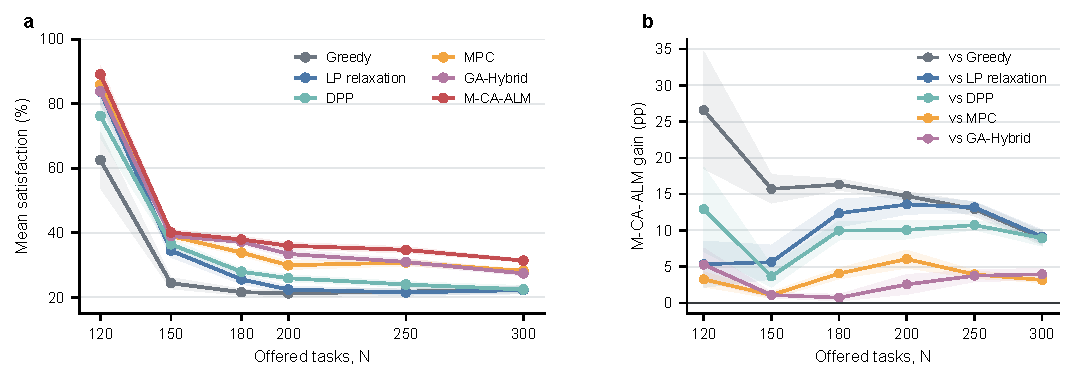
\includegraphics[width=\textwidth]{Fig_Static_Baseline_Comparison.pdf}
\caption{Static baseline comparison.
(a) Mean satisfaction and stored 95\% intervals across 30 paired seeds at
each offered-load level. (b) M-CA-ALM paired satisfaction gain and stored
95\% interval against each implemented baseline. The figure reports only the
fixed five-node simulator and the six tested load levels.}
\label{fig:static_baselines}
\end{figure*}

M-CA-ALM never loses to GA-Hybrid on a paired seed in the six congested scales. Win/tie counts are 28/2 at $N=120$, 25/5 at $N=150$, 14/16 at $N=180$, 24/6 at $N=200$, 28/2 at $N=250$, and 29/1 at $N=300$. The strongest practical effects occur at $N=250$ and $300$, where the paired effect sizes exceed 1.6.

\subsection{Factorial Mechanism Ablation}
We isolate guarded local acceptance ($G$) and repair-aware phenotype ranking ($R$) in a paired $2\times2$ design. Raw disables both factors; Guard enables only $G$; Repair-aware enables only $R$; Full enables both. The four variants use identical environments, solver random streams, final repair, and post-optimization. As an additional reproducibility gate, all 180 Full rows exactly reproduce the corresponding M-CA-ALM rows in the main experiment.

\begin{table}[t]
\centering
\caption{Mean satisfaction (\%) in the 30-seed mechanism ablation.}
\label{tab:official_ablation}
\small
\begin{tabular}{rrrrr}
\toprule
$N$ & Raw & Guard & Repair-aware & Full \\
\midrule
120 & 83.06 & 83.06 & 89.11 & 89.11 \\
150 & 39.69 & 39.69 & 40.11 & 40.11 \\
180 & 36.28 & 36.28 & 37.93 & 37.93 \\
200 & 33.52 & 33.52 & 36.00 & 36.00 \\
250 & 30.65 & 30.65 & 34.71 & 34.71 \\
300 & 27.44 & 27.44 & 31.38 & 31.38 \\
\bottomrule
\end{tabular}
\end{table}

Table~\ref{tab:official_ablation} attributes the observed gain to repair-aware ranking. Its paired main effect ranges from 0.42 to 6.06 percentage points. Full exceeds Raw after Holm correction at five of six scales; $N=150$ is not significant after correcting all ablation comparisons. Guard and Raw are identical on every run, as are Full and Repair-aware, so the estimated guard main effect and interaction are both zero. The guard is therefore a safety invariant in this implementation, not an empirically supported source of higher satisfaction.

\subsection{Cross-Algorithm Transfer and Offline Learned Baseline}
We next test whether repair-aware ranking transfers beyond the ALM search. On independent runs 31--50, GA-Hybrid-Raw and GA-Hybrid-RepairAware use identical environments, evolutionary budgets, random streams, final repair, and post-optimization; only candidate ranking changes. For each run, the paired effect is averaged equally over the six congested scales before inference. Repair-aware GA improves satisfaction by 3.08 points (95\% CI [2.62, 3.68], $d_z=2.48$), wins all 20 run-level pairs, and remains significant after Holm correction. Its scale-wise gain is positive and corrected-significant at every tested $N$, ranging from 1.10 to 4.88 points. The corresponding independent ALM effect is 3.28 points (95\% CI [2.50, 4.40]). This experiment supports repair-aware ranking as an optimizer-independent selection principle within the two tested evolutionary families; it does not establish transfer to arbitrary repair operators.

The learned comparator is a 24-unit bipartite graph policy trained only on runs 51--55, selected only on runs 61--63, and frozen before testing on runs 1--30. The train, selection, and test partitions are disjoint; no test environment updates network parameters or contributes labels. OfflineGNN receives the same final repair, post-optimization, metric code, and paired environments as M-CA-ALM. Its mean satisfaction over $N=120,150,180,200,250,300$ is 74.00\%, 36.27\%, 28.54\%, 26.40\%, 23.80\%, and 22.20\%, respectively. M-CA-ALM is higher at every scale and by 9.67 points after equal scale averaging (95\% CI [8.67, 10.76], $d_z=3.27$; 30/30 run-level wins). Table~\ref{tab:transfer_learning} summarizes the primary paired tests. OfflineGNN is a leakage-free internally trained comparator, not a published method, a new contribution, or a claim of superiority over all learned schedulers.

\begin{table*}[t]
\centering
\caption{Primary paired repair-transfer and offline-learning tests. Effects are satisfaction differences in percentage points after equal averaging over the six congested scales.}
\label{tab:transfer_learning}
\scriptsize
\setlength{\tabcolsep}{2.5pt}
\begin{tabular}{lrrrrrrr}
\toprule
Comparison & Runs & Scales & Mean diff. & 95\% CI & $d_z$ & W/T/L & $p$ \\
\midrule
GA repair-aware $-$ raw & 20 & 6 & 3.08 & [2.62, 3.68] & 2.48 & 20/0/0 & $<0.001$ \\
ALM repair-aware $-$ raw & 20 & 6 & 3.28 & [2.50, 4.40] & 1.41 & 20/0/0 & $<0.001$ \\
M-CA-ALM $-$ OfflineGNN & 30 & 6 & 9.67 & [8.67, 10.76] & 3.27 & 30/0/0 & $<0.001$ \\
\bottomrule
\end{tabular}
\end{table*}

\subsection{Additional Mathematical and Control Baselines}
We add three non-learning comparator baselines under the same final repair and evaluation protocol: an admission-aware LP relaxation with deterministic rounding (LPRelax), a deadline-ordered dynamic placement heuristic (DPP), and a short-horizon rollout controller (MPC). The LP solves a linear memory/load proxy and is not treated as an exact optimum for the nonlinear simulator. Table~\ref{tab:official_baselines} reports the mean satisfaction for all six compared methods at the congested scales.

\begin{table*}[t]
\centering
\caption{Mean satisfaction (\%) with additional static baselines (30 paired seeds per scale).}
\label{tab:official_baselines}
\small
\begin{tabular}{rrrrrrr}
\toprule
$N$ & Greedy & GA-Hybrid & LPRelax & DPP & MPC & M-CA-ALM \\
\midrule
120 & 62.53 & 83.83 & 83.78 & 76.19 & 85.86 & 89.11 \\
150 & 24.38 & 39.02 & 34.49 & 36.44 & 39.02 & 40.11 \\
180 & 21.59 & 37.20 & 25.56 & 27.94 & 33.87 & 37.93 \\
200 & 21.25 & 33.45 & 22.42 & 25.93 & 29.95 & 36.00 \\
250 & 21.77 & 30.96 & 21.52 & 23.97 & 30.77 & 34.71 \\
300 & 22.44 & 27.42 & 22.26 & 22.44 & 28.21 & 31.38
 \\
\bottomrule
\end{tabular}
\end{table*}

M-CA-ALM is higher than every comparator on every scale in the paired means. The five paired comparisons at each scale remain significant after Holm correction over all 30 ALM-versus-baseline tests; the largest adjusted value is $0.0015$. MPC is the strongest low-cost competitor at high load, but remains 3.17 percentage points below M-CA-ALM at $N=300$ while running roughly 50 times faster. This comparison exposes the practical trade-off rather than hiding it: the proposed method buys satisfaction with second-scale computation, whereas MPC is preferable when latency budget dominates.

\subsection{Admission and Runtime Trade-off}
Admission is 100\% through $N=200$. At $N=250$, mean admission is 93.25\% for M-CA-ALM and 93.28\% for GA-Hybrid; at $N=300$, it is 86.94\% and 86.89\%, respectively. Satisfaction gains therefore do not come from materially more aggressive admission.

M-CA-ALM is consistently slower. Its mean runtime is 3.10--3.18 times that of GA-Hybrid, increasing from 0.50~s at $N=120$ to 1.11~s at $N=300$. GA-Hybrid increases from 0.16~s to 0.35~s. This cost is compatible with the measured second-scale simulation windows, but it is not evidence for millisecond scheduling or deployment latency.

The equal-budget control changes the interpretation of the primary comparison. At $N=120,150,180,200,300$, the ALM--GA-Hybrid paired mean differences are $-4.00$, $-1.07$, $-0.67$, $+0.10$, and $-0.07$ percentage points, respectively; at $N=250$ the difference is $+2.32$ points. The five-run control is therefore mixed rather than uniformly favorable to M-CA-ALM. Its ALM runtime is approximately 3.4--4.3 times the GA-Hybrid runtime. These results prevent the fixed-configuration advantage from being attributed solely to a method advantage under equal computation; the supported claim is that repair-aware ALM can be effective in the tested congested regime, with substantial computation cost and load-dependent outcome.

\subsection{State-Preserving Replay and the Overload Boundary}
We next embed Greedy, GA-Hybrid, and M-CA-ALM in a separate 500-slot state-preserving replay at $N\in\{180,300\}$. Each scale uses 20 paired environment runs. Unresolved tasks retain their identities across slots, the backlog is capped at $N$, and all methods observe the same arrivals and environment seed in each paired run. This replay is a dynamic experiment with carry-over state and repeated arrivals, not a temporal extension of the one-shot static experiment; its observations are therefore analyzed separately. The replay contains 60,000 slot records and 120 run records. Before analysis, validation checks duplicate keys, complete slot coverage, algorithm pairing, seed matching, and resource feasibility.

\begin{table}[t]
\centering
\caption{State-preserving 500-slot replay results (20 paired runs per scale). Saturation is the first slot with backlog equal to its cap.}
\label{tab:official_replay}
\scriptsize
\begin{tabular}{llrrr}
\toprule
$N$ & Method & Mean sat. & Median full slot & Queue drops \\
\midrule
180 & Greedy & 28.70 & 3 & 38,280 \\
180 & GA-Hybrid & 33.45 & 7 & 30,486 \\
180 & M-CA-ALM & \textbf{46.41} & \textbf{56} & \textbf{24,550} \\
300 & Greedy & 3.78 & 2 & 138,535 \\
300 & GA-Hybrid & \textbf{8.97} & 2 & \textbf{122,994} \\
300 & M-CA-ALM & 3.51 & 2 & 139,345 \\
\bottomrule
\end{tabular}
\end{table}

At $N=180$, M-CA-ALM exceeds GA-Hybrid by 12.96 percentage points in mean satisfaction (95\% CI [5.79, 20.12], $d_z=0.79$), wins all 20 paired runs, and remains significant after Holm correction ($p=0.00080$). Its median first full-backlog slot is 56, compared with 7 for GA-Hybrid and 3 for Greedy; one ALM run never reaches the cap. Thus, the dynamic benefit is expressed not only in slot satisfaction but also in delayed queue saturation and fewer queue-cap drops.

The $N=300$ replay defines a different operating regime. Every method reaches the backlog cap at slot 2 in every run. M-CA-ALM averages 3.51\% satisfaction, compared with 8.97\% for GA-Hybrid and 3.78\% for Greedy. The ALM--GA difference is negative, but does not remain significant after family-wise Holm correction ($p=0.152$). We therefore treat $N=300$ as an immediate-overload boundary, not as evidence of dynamic superiority. Figure~\ref{fig:replay_overload} shows how this boundary changes both cumulative completions and queue-cap losses.

\begin{figure*}[t]
\centering
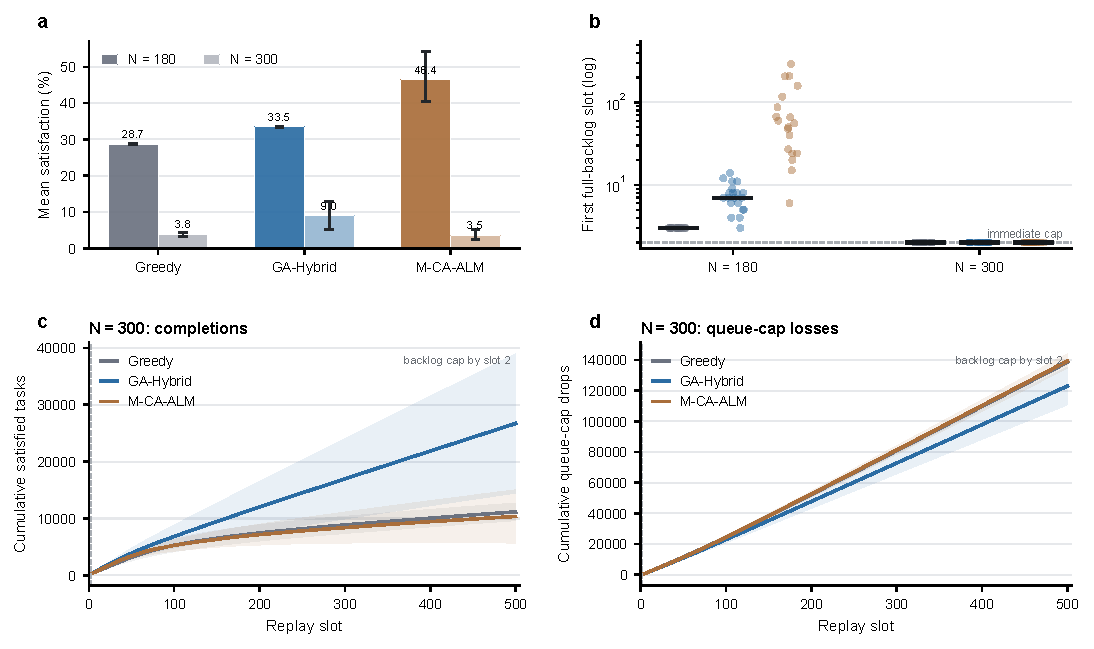
\includegraphics[width=\textwidth]{Fig_Replay_Overload_Boundary.pdf}
\caption{Static-to-dynamic operating boundary. (a) Mean slot satisfaction with run-level 95\% confidence intervals. (b) First full-backlog slot for each paired run; black lines indicate medians and the vertical axis is logarithmic. (c) Cumulative satisfied tasks at $N=300$. (d) Cumulative queue-cap drops at $N=300$. Bands in (c)--(d) are 95\% confidence intervals over 20 runs. At $N=300$, all methods reach the backlog cap at slot 2, so the result bounds rather than extends the recoverable-congestion claim.}
\label{fig:replay_overload}
\end{figure*}

\section{Discussion}

\subsection{Why Outcome Alignment Matters}
The original solver ranked raw assignments and repaired only after search. That design produced almost no confirmed advantage over GA-Hybrid. Repair-aware ranking changes the search signal: a genotype is valuable only when its deployed phenotype increases the satisfied-task count. Preserving the unrepaired genotype avoids turning repair into a population-wide template. The factorial ablation directly supports this interpretation: Repair-aware and Full are identical on all 180 paired environments, whereas Raw and Guard are also identical. Independent GA-family tests then reproduce a positive repair-aware effect at all six congested scales. The improvement is therefore attributable to outcome-aligned ranking rather than to the acceptance guard, a different final feasibility rule, or an ALM-specific update.

\subsection{Regime Dependence}
The static protocol begins at $N=120$; lower offered-load cells were not
part of the reported experiment. Within the tested scales, the benefit is largest at $N=250$ and 
$N=300$. This pattern is consistent with the proposed mechanism: 
repair-aware ranking carries little information when almost every candidate 
is satisfiable, but becomes discriminative when raw structural differences 
determine which tasks survive repair.

\subsection{Cost and Deployment Scope}
The improved satisfaction requires repeated repair evaluations during evolution. M-CA-ALM is roughly three times slower than GA-Hybrid and far slower than Greedy. It is suitable for centralized orchestration with second-scale decision windows, but the present implementation is not an ultra-low-latency scheduler. The zero guard effect also suggests that its current role is defensive: it enforces monotone local acceptance but does not improve the tested outcomes. The runtime overhead is therefore a measured limitation of the present implementation rather than evidence for a broader real-time deployment claim.

\subsection{Dynamic Operating Boundary}
The replay results show why static congestion and dynamic overload must be distinguished. At $N=180$, M-CA-ALM delays median queue saturation from slot 7 to slot 56 relative to GA-Hybrid while increasing satisfaction and reducing queue-cap drops. This is consistent with outcome-aligned selection preserving more useful service capacity across repeated decisions. The $N=300$ replay is qualitatively different: the queue is full by slot 2 for every controller and every run. Once the system enters this immediate-saturation regime, the slot-local repair-aware objective no longer guarantees the best cumulative throughput, and GA-Hybrid completes more tasks on average.

This negative boundary is not inconsistent with the static $N=300$ result. The static experiment evaluates one repaired batch, whereas replay repeatedly adds arrivals to unresolved work. Under the present fixed capacity, the latter creates a demand level at which almost no transient recovery interval remains. The result therefore supports a regime-dependent claim: M-CA-ALM is effective in recoverable congestion, whereas persistent immediate saturation lies outside the operating range established here.

\subsection{Limitations}
The formal experiment uses one fixed five-node infrastructure and trace-driven simulation. It does not establish generalization to other node ratios, mobility patterns, packet-level contention, or live hardware clusters. The primary baseline comparison is fixed-configuration rather than equal-budget: GA-Hybrid receives $100\times100$ evolutionary iterations and M-CA-ALM receives $50\times50$. The equal-budget control is mixed across load levels and has a 3.4--4.3-fold ALM runtime penalty, so the fixed-table superiority must not be presented as a budget-normalized universal result. The repair-transfer result is scoped to the tested Safe Harbor repair operator and the two tested evolutionary families; it is not evidence for arbitrary repair operators. The low-load ceiling also reduces the number of informative static scales. The comparison includes Greedy, GA-Hybrid, LPRelax, DPP, MPC, M-CA-ALM, and a split-isolated OfflineGNN, but one frozen graph policy does not represent the full space of learned schedulers. The tested task-count axis is not a cross-infrastructure load measure. These limitations bound the evidence to the stated simulator, topology, algorithms, repair operator, search configurations, and operating regimes; they do not support online-stability, capacity-planning, or deployment claims.

\section{Conclusion}

This paper identifies and addresses an objective mismatch in repair-based fog scheduling: raw candidates are often optimized even though only repaired phenotypes are deployed. The proposed M-CA-ALM ranks candidates by repaired outcome while preserving unrepaired genotypes for diversity and guarding local ALM refinement against regressions.

In a frozen five-node benchmark with 30 paired seeds at six tested scales
$N\in\{120,150,180,200,250,300\}$, the fixed-configuration method improves
satisfaction at every tested congested scale. The confirmed gain ranges from
0.72 to 5.28 percentage points; all six fixed-configuration comparisons remain
significant after Holm correction, and no paired seed favors GA-Hybrid. A
separate five-run equal-budget control is mixed across scales, so the primary
result is not a budget-normalized superiority claim. At $N=300$, satisfaction
increases from 27.42\% to 31.38\% in the primary configuration, with a large
paired effect size and an approximately threefold runtime increase.

A separate 30-seed factorial ablation attributes the performance change to repair-aware phenotype ranking: enabling the ranking changes mean satisfaction by 0.42--6.06 percentage points across congested scales, whereas guarded acceptance has zero measured main or interaction effect. We therefore retain the guard as a monotone safety condition rather than claim it as a performance-producing component.

Independent runs 31--50 reproduce the ranking effect in GA-Hybrid: the run-averaged repair-aware gain is 3.08 points across six congested scales, with all 20 paired run effects positive. A separately trained and frozen OfflineGNN remains 9.67 points below M-CA-ALM after equal scale averaging on the 30 test runs. These controls broaden the evidence beyond the original ALM ablation while remaining limited to one shared repair operator and one offline learned architecture.

Formal 500-slot replay further bounds the claim. At $N=180$, M-CA-ALM improves mean satisfaction from 33.45\% to 46.41\%, wins all 20 paired runs, delays median full-backlog onset from slot 7 to slot 56 relative to GA-Hybrid, and reduces queue-cap drops. At $N=300$, however, all controllers reach the backlog cap by slot 2 and M-CA-ALM no longer leads. The method is therefore supported in recoverable congestion, not under arbitrary overload.

The supported conclusion is correspondingly narrow: repair-aware outcome alignment improves both tested evolutionary families in the reported fixed-topology benchmark, with a measured runtime cost and a documented immediate-saturation boundary. The present results do not establish transfer to arbitrary repair operators, cross-infrastructure generalization, online stability, capacity planning, or live deployment.

\begin{appendices}
\section{Implementation Notes}

\subsection{Local Search Objective}
The MATLAB implementation applies short augmented-Lagrangian style updates inside a relaxed assignment space. The local objective combines a smooth deadline-satisfaction surrogate with penalty terms for deadline pressure and assignment consistency:
\begin{equation}
    \mathcal{L}(\mathbf{P}, \boldsymbol{\lambda}, \rho) =
    f(\mathbf{P}) + \sum_k \psi_k(\mathbf{P}, \lambda_k, \rho)
\end{equation}
where $f(\mathbf{P})$ denotes the negative surrogate utility and $\psi_k$ represents the penalty terms used in the current implementation. This appendix should be interpreted as an implementation-oriented summary rather than a formal convergence proof for the full memetic solver, because the complete algorithm also includes crossover, mutation, repair, and discrete post-optimization.

\subsection{Static Batch Congestion Derivative}
\label{appendix:gradients}
The continuous local search uses the same static batch congestion structure as the main text. For a node $f$, define
\begin{equation}
    \rho_f = \frac{\sum_i p_{i,f}\,\mathrm{Comp}_{i,f}}{\bar{T}}
\end{equation}
and for the stable region $\rho_f < 0.99$ use
\begin{equation}
    q_f(\rho_f) = 1 + \frac{\rho_f}{2(1-\rho_f+\epsilon)}.
\end{equation}
The corresponding sensitivity with respect to $\rho_f$ is
\begin{equation}
    \frac{\partial q_f}{\partial \rho_f}
    =
    \frac{1+\epsilon}{2(1-\rho_f+\epsilon)^2},
\end{equation}
which is well approximated in code by the dominant term $\frac{1}{2(1-\rho_f)^2}$ when $\epsilon$ is very small. Combining this with
\begin{equation}
    \frac{\partial \rho_f}{\partial p_{k,f}} = \frac{\mathrm{Comp}_{k,f}}{\bar{T}}
\end{equation}
gives a node-level gradient signal that becomes steep near saturation. This is the mechanism used to discourage the relaxed search from adding probability mass to already congested nodes.

\subsection{Softmax Relaxation}
\label{appendix:relaxation}
To support gradient-based updates, the solver maps logits to per-task assignment probabilities:
\begin{equation}
    p_{i,f} = \frac{e^{z_{i,f}}}{\sum_{j=1}^{M} e^{z_{i,j}}}.
\end{equation}
This mapping keeps each task on the probability simplex during local refinement. The final binary decision is then recovered by an argmax projection, after which repair and discrete post-optimization are applied.

\subsection{Repair and Post-Processing Cost}
\label{appendix:complexity}
The repair stage checks each task against candidate nodes and may scan all fog nodes when the original placement is infeasible. Under this implementation, one repaired solution therefore has worst-case cost $O(NM)$. The subsequent discrete post-optimization pass reuses the repaired assignment and attempts local reassignment improvements, so its cost is of the same order per sweep.

\subsection{Per-Generation Cost Summary}
One generation of M-CA-ALM combines several components:
\begin{itemize}
    \item precomputed matrix reuse for communication and computation costs;
    \item local-search updates on a subset of the population;
    \item feasibility-first evaluation and tournament selection;
    \item integer crossover, mutation, repair, and elitism.
\end{itemize}
Using the notation of Section~4, the dominant cost per generation is governed by local-search and repair operations, which is consistent with the practical scaling discussion in the main text. This appendix does not claim a formal global runtime bound for all implementation branches; it summarizes the main computational terms observed in the current code.
\end{appendices}


\backmatter
\section*{Declarations}
\begin{description}
\item[Funding] Author confirmation required before submission.
\item[Competing interests] Author confirmation required before submission.
\item[Data availability] Frozen run-level data, figure source data, solver
code, and checksum manifests are included in the reproducibility package.
The authors must insert the public repository DOI or URL before submission.
\item[Code availability] Author confirmation of the repository DOI or URL is
required before submission.
\item[Author contributions] CRediT roles must be completed and approved by
all authors before submission.
\item[Ethics approval and consent to participate] Not applicable to
simulator-only experiments.
\item[Consent for publication] Not applicable.
\end{description}

\bibliography{references}
\end{document}
